
% This work is licensed under the Creative Commons Attribution-Share Alike 2.0 France License.
% To view a copy of this license, visit http://creativecommons.org/licenses/by-sa/2.0/fr/legalcode
% or send a letter to Creative Commons, 171 Second Street, Suite 300, San Francisco, California, 94105, USA.


\chapter{Comment poser une question}

Attention l'ensemble des exemples de ce chapitre sont entourés de vert car il faut copier avec exactitude les espaces ajoutées dans ces codes. Toutes les indentations de ce chapitre sont composées de quatre espaces (quatre appuis sur la barre d'espace). Ces indentations définissent des blocs que nous verrons dans le chapitre suivant.

Si vous n'entrez pas les espaces correctement vous pourriez avoir une erreur du type:

\begin{Verbatim}[frame=single,rulecolor=\color{red}, label=erreur]
IndentationError: expected an indented block
\end{Verbatim}

\setsansfont[Mapping=tex-text]{DejaVu Sans}
Les espaces que ce soient des espaces normales ou des tabulations «~\textsf{⇆}~» sont extrêmement  importantes en Python. Nous en parlerons en détail dans le chapitre suivant.

\section{Avec des «~si~» on mettrait Paris en bouteille}
En termes de programmation, une question signifie usuellement que nous voulons faire des choses différentes selon 
la réponse à la question. Cela est appelé un «~test si~».

Par exemple:

\emph{Quel âge avez-vous ? Si vous avez plus que 18 ans, vous êtes majeur !}\\


Cela peut être écrit en Python avec le «~\texttt{test si}~» suivant:
\begin{Verbatim}[frame=single,rulecolor=\color{gray}, label=ne pas saisir]
if âge > 18:
    print('Vous êtes majeur !')
\end{Verbatim}

Une représentation graphique peut être observée figure \ref{fig:Cf-if-fr}.

\begin{figure}[ht]
\centering
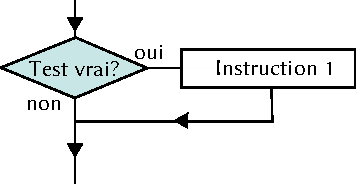
\includegraphics[scale=1.5]{images/Cf-if-fr.pdf}
\caption{Diagramme d'un test «~si~»}
\label{fig:Cf-if-fr}
\end{figure}

Un test \emph{si} est fait d'un «~\texttt{if\footnote{Le mot \emph{if} signifie «~si~» en français.}}~» suivit de ce que nous appelons une «~condition~»  (plus de  détails dans une seconde) suivit par deux points «~\verb+:+~». Les lignes qui suivent le «~\texttt{if}~» doivent constituer un bloc; si la réponse à la question est «~oui~» (ou «~vrai~» comme nous le disons en termes de programmation) alors les commandes dans le bloc sera exécutées.\\

Une condition est élément de programmation qui retourne «~oui~» (vrai) ou «~non~» (faux). Il y a certains symboles (ou opérateurs) qui sont utilisés pour créer des conditions, comme dans la table \ref{table:opcond}:

\begin{table}[h!]
\begin{center}
\begin{tabular}{|c|c|}
\hline
\texttt{Opérateur}&Opération\\
\hline
\texttt{==}&Égal\\
\hline
\texttt{!=}&Différent\\
\hline
\texttt{>}&Plus grand que\\
\hline
\texttt{<}&Plus petit que\\
\hline
\texttt{>=}&Plus grand ou égal à\\
\hline
\texttt{<=}&Plus petit ou égal à\\
\hline
\end{tabular}
\end{center}
\caption{Opérateurs de condition}
\label{table:opcond}
\end{table}

Par exemple si vous avez 10 ans alors la condition «~\texttt{votre\_âge == 10}~» retournera vrai (oui). Si vous n'avez pas dix ans  elle retournera faux. \\

\fcolorbox{black}{lbleu}{
\centering\begin{minipage}{0.9\textwidth}
Rappelez-vous: ne confondez pas les \emph{deux} symboles égal utilisés dans une condition «~\texttt{==}~», avec le signe égal utilisé pour assigner une variable. Si vous utiliser un seul symbole «~\texttt{=}~» dans une condition, vous obtiendrez un message d'erreur.\end{minipage}}
\\


Présumons que vous avez attribué votre âge à une variable «~\texttt{âge}~»  et bien si vous avez douze ans la condition «~\texttt{âge > 10}~» sera \emph{vraie}.

Si vous avez huit ans elle retournera \emph{faux}.
Si vous avez dix ans elle retournera \emph{faux} car la condition est vérifiée pour \emph{strictement} plus grand «~\texttt{>}~»  que dix et non pas pour plus grand ou égal «~\texttt{>=}~» à dix.\\

Essayons quelques exemples:

\begin{Verbatim*}[frame=single,rulecolor=\color{green}, label=à taper avec attention]
>>> âge = 10
>>> if âge > 10:
...     print('Arrivé ici !')
\end{Verbatim*}

Si vous avez obtenu une erreur c'est que vous avez oublié quelques espaces (que je vous montre ici en les remplaçant par des @):

\begin{Verbatim}[frame=single,rulecolor=\color{gray}, label=ne pas saisir]
>>> âge = 10
>>> if âge > 10:
... @@@@print('Arrivé ici !')
\end{Verbatim}

Si vous entrez l'exemple ci dessus dans une console qu'arrivera-t-il?\\

\emph{Rien!}\\

Parce que la valeur de la variable «~\texttt{âge}~» n'est pas strictement plus grande que dix, la commande «~\texttt{print}~» dans le bloc ne sera pas lancée. Maintenant étudions:

\begin{Verbatim}[frame=single,rulecolor=\color{green}, label=à taper avec attention]
>>> âge = 10
>>> if âge >= 10:
...     print('Arrivé ici !')
Arrivé ici !
\end{Verbatim}

Si nous essayons cet exemple, alors nous pouvons voir le message affiché. La même chose arrivera avec l'exemple suivant:

\begin{Verbatim}[frame=single,rulecolor=\color{green}, label=à taper avec attention]
>>> âge = 10
>>> if âge == 10:
...     print('Arrivé ici !')
Arrivé ici !
\end{Verbatim}

\begin{center}

\includegraphics[scale=1]{images/paris.pdf}
\end{center}

\section{Fait cela! Ou sinon...}

Nous pouvons aussi étendre un test «~si~» et faire quelque chose quand la condition n'est pas vraie. Par exemple, afficher le mot «~Bonjour~» sur la console si votre âge est de douze ans mais «~Au revoir~»  s'il est différent. Pour faire cela nous utilisons in test «~si sinon~», ce qui est une autre manière de dire «~si quelque chose est vrai fait cela sinon fait ça~»:

\begin{Verbatim}[frame=single,rulecolor=\color{green}, label=à taper avec attention]
>>> âge = 12
>>> if âge == 12:
...     print('Bonjour !')
... else:
...     print('Au revoir !')
Bonjour !
\end{Verbatim}

Le test «~si sinon~» utilise «~\texttt{if}~» pour si et «~\texttt{else\footnote{Le mot \emph{else} signifie «~sinon~» et provient du latin \emph{alius} (autre) et \emph{alter} (l'autre de deux).}}~» pour sinon.

Rentrez l'exemple ci-dessus et vous devriez voir «~\texttt{Bonjour !}~» affiché dans la console.
Changez la valeur de la variable «~\texttt{âge}~»  à une autre valeur et «~\texttt{Au revoir !}~»  sera affiché:

\begin{Verbatim}[frame=single,rulecolor=\color{green}, label=à taper avec attention]
>>> âge = 8
>>> if âge == 12:
...     print('Bonjour !')
... else:
...     print('Au revoir !')
Au revoir !
\end{Verbatim}

Une représentation graphique peut être observée figure \ref{fig:Cf-else-fr}.

\begin{figure}[ht]
\centering
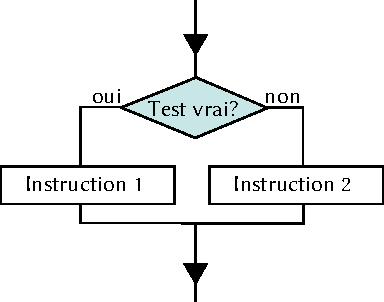
\includegraphics[scale=1.5]{images/Cf-else-fr.pdf}
\caption{Diagramme d'un test «~si~»}
\label{fig:Cf-else-fr}
\end{figure}


\section{Fait cela, ou cela, ou cela! Ou sinon...}
Nous pouvons étendre le test «~si~» encore plus loin en utilisant «~\texttt{elif}~» (l'abréviation  de else-if, «~sinon, si~»). Par exemple, nous pouvons vérifier si votre âge est égal à dix, puis à onze, puis à douze et ainsi de suite: 

\begin{Verbatim}[frame=single,rulecolor=\color{green}, label=à taper avec attention]
>>> âge = 12
>>> if âge == 10:
...     print('Vous avez 10 ans.')
... elif âge == 11:
...     print('Vous avez 11 ans.')
... elif âge == 12:
...     print('Vous avez 12 ans.')
... elif âge == 13:
...     print('Vous avez 13 ans.')
... else:
...     print('Je ne connais pas votre âge.')
Vous avez 12 ans.
\end{Verbatim}

Dans le code ci-dessus, le code vérifie à la deuxième ligne si la valeur de la variable «~\texttt{âge}~» est égale à dix.
Si elle ne l'est pas alors il saute à la quatrième ligne pour vérifier si 
la valeur de la variable «~\texttt{âge}~» est égale à onze. À nouveau  celle-ci     ne l'est pas donc il saute à la sixième ligne  pour vérifier si 
la valeur de la variable «~\texttt{âge}~» est égale à douze. Dans ce cas cela est le cas donc Python va dans le bloc à la septième ligne et exécute la commande «~\texttt{print}~».
Vous avez probablement remarqué qu'il a cinq groupes dans ce code aux lignes 3, 5, 7, 9 et 11.

Une représentation graphique peut être observée figure \ref{fig:Cf-elif-fr}.

\begin{figure}[ht]
\centering
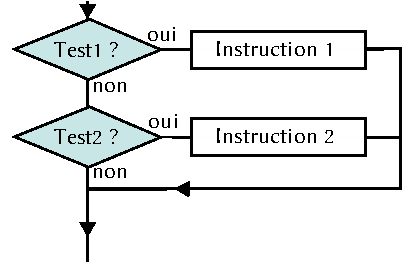
\includegraphics[scale=1.5]{images/Cf-elif-fr.pdf}
\caption{Diagramme d'un test «~si~»}
\label{fig:Cf-elif-fr}
\end{figure}

\section{Combiner des conditions}
Vous pouvez combiner des conditions ensemble en utilisant les mots clefs «~\texttt{and}~» qui signifie «~et~» et «~\texttt{or}~» qui signifie «~ou~».

Nous pouvons condenser l'exemple précédent, un petit peu, en utilisant «~\texttt{or}~» pour joindre les conditions ensemble:

\begin{Verbatim}[frame=single,rulecolor=\color{green}, label=à taper avec attention]
>>> if âge == 10 or âge == 11 or âge == 12 or âge == 13:
...     print('Vous avez %s ans.' % âge)
... else:
...     print('Heu ?')
\end{Verbatim}

Si n'importe laquelle des conditions de la première ligne est vraie, c'est à dire si  «~\texttt{âge}~» est égal à 10, 11, 12 ou 13, alors le bloc de code ligne 2 sera exécuté. Sinon Python ira à la quatrième ligne. 
Nous pouvons condenser ce code un peu plus en utilisant les opérateurs «~\texttt{and}~», «~\texttt{>=}~», «~\texttt{<=}~»:

\begin{Verbatim}[frame=single,rulecolor=\color{green}, label=à taper avec attention]
>>> if âge >= 10 and âge <= 13:
...     print('Vous avez %s ans.' % âge)
... else:
...     print('Heu ?')
\end{Verbatim}

Vous avez probablement compris que si les deux conditions de la première ligne sont vraies alors le bloc de la deuxième ligne est exécuté (si «~\texttt{âge}~»  est plus grand ou égal à dix et «~\texttt{âge}~» est plus petit ou égal à 13. Donc si la variable «~\texttt{âge}~» vaut douze alors «~\texttt{Vous avez 12 ans.}~» sera affiché sur la console parce que douze est plus grand que dix et plus petit que treize.

\section{Rien}
Il y a une autre sorte de valeur qui peut être assignée à une variable et dont nous n'avons pas encore parlé dans les chapitres précédents: \textbf{rien}!

De la même manière que les nombres, les chaînes et les listes peuvent être assignés à des variables «~{rien}~»   est aussi un type de valeur qui peut être assigné. En Python une valeur vide est désignée comme «~\texttt{None\footnote{Le mot \emph{none} signifie aucun, personne en anglais, contraction de \emph{no one} pas un.}}~».

Une variable valant «~\texttt{None}~» (dans d'autres langages, «~\texttt{null}~» est parfois utilisé) peut être utilisée comme les les autres variables:

\begin{Verbatim}[frame=single,rulecolor=\color{mbleu}, label=à taper]
>>> maval = None
>>> print(maval)
None
\end{Verbatim}

\begin{center}
\textcolor{blue}{\textrm{\scalefont{5}\{\}==∅==None}}
\end{center}

«~\texttt{None}~» est une manière de réinitialiser une variable comme étant non utilisée ou une manière de créer une variable sans fixer sa valeur avant de l'utiliser.

Par exemple si votre équipe de football lève des fonds pour de nouveaux uniformes, vous voulez peut-être attendre que toute l'équipe soit revenue avec l'argent récoltée avant d'ad\-di\-tion\-ner les montants. En termes de programmation, vous pouvez avoir une variable pour chaque joueur de l'équipe et initialiser ces variables à «~\texttt{None}~»:

\begin{Verbatim}[frame=single,rulecolor=\color{mbleu}, label=à taper]
>>> joueur1 = None
>>> joueur2 = None
>>> joueur2 = None
\end{Verbatim}

Nous pouvons utiliser un test «~si~» pour vérifier ces variables de manière à déterminer si tous les membres de l'équipe sont revenus avec l'argent qu'ils ont levé:

\begin{Verbatim}[frame=single,rulecolor=\color{green}, label=à taper avec attention]
>>> if joueur1 is None or joueur2 is None or joueur3 is None:
...     print('''S'il-vous-plait, attendez jusqu'à ce 
...que tous les joueurs soient revenus.''')
... else:
...     print('Vous avez levé %s€' % (player1 + player2 + player3))
\end{Verbatim}

Le test «~si~» contrôle si une des variables a une valeur nulle et affiche le premier message si cela est la cas.

Le mot \emph{is} est la troisième personne du verbe \emph{to be}, c'est à dire être en français. Le test est donc «~Est ce que joueur1, joueur2 ou joueur3 sont nuls?~». 

Si chaque variable a une valeur non nulle alors le second message est affiché avec la somme totale récoltée.
Si vous essayez le code avec toutes les variables qui pointent vers «~\texttt{None}~»,  vous aurez le premier message (n'oubliez pas de créer les variables d'abord ou vous aurez un message d'erreur):

\begin{Verbatim}[frame=single,rulecolor=\color{green}, label=à taper avec attention]
>>> if joueur1 is None or joueur2 is None or joueur3 is None:
...     print('''S'il-vous-plait, attendez jusqu'à ce 
...que tous les joueurs soient revenus.''')
... else:
...     print('Vous avez levé %s€' % (player1 + player2 + player3))
S'il-vous-plait, attendez jusqu'à ce 
que tous les joueurs soient revenus.
\end{Verbatim}

Même si vous avez modifié une ou deux variables, vous continuerez d'avoir le même message:

\begin{Verbatim}[frame=single,rulecolor=\color{green}, label=à taper avec attention]
>>> joueur1=100
>>> joueur2=300
>>> if joueur1 is None or joueur2 is None or joueur3 is None:
...     print('''S'il-vous-plait, attendez jusqu'à ce 
...que tous les joueurs soient revenus.''')
... else:
...     print('Vous avez levé %s€' % (player1 + player2 + player3))
S'il-vous-plait, attendez jusqu'à ce 
...que tous les joueurs soient revenus.
\end{Verbatim}

Finalement une fois toutes les variables modifiées vous verrez le message du second bloc:

\begin{Verbatim}[frame=single,rulecolor=\color{green}, label=à taper avec attention]
>>> joueur1=100
>>> joueur2=300
>>> joueur3=400
>>> if joueur1 is None or joueur2 is None or joueur3 is None:
...     print('''S'il-vous-plait, attendez jusqu'à ce 
...que tous les joueurs soient revenus.''')
... else:
...     print('Vous avez levé %s€' % (player1 + player2 + player3))
Vous avez levé 800€
\end{Verbatim}

\section{Quelle est la différence?\label{sec:dif}}

Quelle est la différence entre «~\texttt{«~10~»}~» et «~\texttt{'10'}~»?
Pas grande mis à part les apostrophes, pouvez-vous penser. Et bien, si vous avez bien lu les chapitres précédents vous savez que le premier est un nombre et que le second est une chaîne. Cela les rend plus différents que ce à quoi vous pourriez vous attendre. Auparavant nous avions comparé la valeur de la variable «~\texttt{âge}~» à un nombre dans un test «~si~»:

\begin{Verbatim}[frame=single,rulecolor=\color{green}, label=à taper avec attention]
>>> if âge == 10:
...     print('Vous avez 10 ans.')
\end{Verbatim}

Si vous aviez attribué dix à la variable «~\texttt{âge}~»  la fonction «~\texttt{print}~»  sera appelée:

\begin{Verbatim}[frame=single,rulecolor=\color{green}, label=à taper avec attention]
>>> âge = 10
>>> if âge == 10:
...     print('Vous avez 10 ans.')
...
Vous avez 10 ans.
\end{Verbatim}

Mais si «~\texttt{âge}~»  a pour valeur «~\texttt{"10"}~» alors la fonction «~\texttt{print}~» ne sera pas appelée:

\begin{Verbatim}[frame=single,rulecolor=\color{green}, label=à taper avec attention]
>>> âge = '10'
>>> if âge == 10:
...     print('Vous avez 10 ans.')
...
\end{Verbatim}

Pourquoi le code dans le bloc n'a pas été exécuté? Parce qu'une chaîne est différente d'un nombre, même s'ils se ressemblent:

\begin{Verbatim}[frame=single,rulecolor=\color{mbleu}, label=à taper]
>>> âge1 = 10
>>> âge2 = '10'
>>> print(âge1)
10
>>> print(âge2)
10
\end{Verbatim}

Regardez! Ils semblent exactement identiques. Pourtant, parce que l'un est une chaîne et l'autre est un nombre, ils ont des valeurs différentes. Néanmoins après «~\texttt{âge="10"}~», «~\texttt{âge == 10}~»  sera toujours faux tant qu'«~\texttt{âge}~» sera une chaîne.  Nous sommes trompés par Python dont la fonction «~\texttt{print}~» est capable de convertir un nombre en chaîne pour l'afficher.

\begin{center}

\includegraphics[scale=1]{images/livre.pdf} 
\end{center}

Il probablement une meilleure manière de penser les choses: c'est de considérer dix livres et dix briques. Le nombre d'éléments peut être le même mais vous ne diriez pas que dix livres sont exactement la même chose que dix briques, n'est-ce-pas? Par chance, en Python nous avons des fonctions magiques qui peuvent transformer des chaînes en nombres et des nombres en chaînes même si elles ne peuvent pas vraiment transformer les briques en livres. Par exemple, pour convertir la chaine «~\texttt{'10'}~»  en un nombre vous pouvez utiliser la fonction «~\texttt{int}~»: 

\begin{Verbatim}[frame=single,rulecolor=\color{mbleu}, label=à taper]
>>> âge_en_chaîne = '10'
>>> âge_en_nombre = int(âge)
>>> print(âge_en_chaîne*2)
1010
>>> print(âge_en_nombre*2)
20
\end{Verbatim}

L'abbreviation «~\texttt{int}~»  est utilisé  pour \emph{integer} qui signifie entier en anglais. C'est-à-dire un nombre entier (sans virgule).\\

La variable «~\texttt{âge\_en\_nombre}~» contient le nombre dix et pas une chaîne. Pour convertir un nombre en une chaîne, vous pouvez utiliser la fonction «~\texttt{str}~»:

\begin{Verbatim}[frame=single,rulecolor=\color{mbleu}, label=à taper]
>>> âge_en_nombre = 10
>>> âge_en_chaîne = str(âge_en_nombre)
\end{Verbatim}

L'abréviation «~\texttt{str}~» est utilisé en lieu de \emph{string} qui signifie ficelle en anglais mais plus particulièrement chaîne de caractères en programmation\footnote{L'appellation française est pour une fois nettement plus compréhensible que la forme originale en anglais.}.\\

«~\texttt{âge\_en\_chaîne}~» contient la chaîne «~\texttt{'10'}~» et non pas un nombre. Revenons à notre test «~si~» qui n'imprimait rien:

\begin{Verbatim}[frame=single,rulecolor=\color{green}, label=à taper avec attention]
>>> âge = '10'
>>> if âge == 10:
...     print('Vous avez dix ans.')
...
\end{Verbatim}

Si nous convertissons la variable avant le test alors nous aurons un résultat différent:

\begin{Verbatim}[frame=single,rulecolor=\color{green}, label=à taper avec attention]
>>> âge = '10'
>>> âge_converti=int(âge)
>>> if âge_converti == 10:
...     print('Vous avez dix ans.')
...
Vous avez dix ans.
\end{Verbatim}



\clearemptydoublepage